\chapter{新闻事件的可视化方法设计}

\section{Storyline 方法研究}
Storyline 是指描述的是人物之间随时间变化的社交关系,它将这些复杂的信息在一张图形上展现出来。该可视化方法最早是由 Mounroe 提出,并发布在著名漫画网站 XKCD 的 "Movie Narrative Charts" \cite{xkcd657} 中。在这个连载漫画中,手绘的 Storyline 用于概括电影中角色之间的互动。Figure.\ref{xkcd} 正是摘自 XKCD 网站。
% BEGIN == XKCD 手绘图
\begin{figure}[htb]
	\centering
		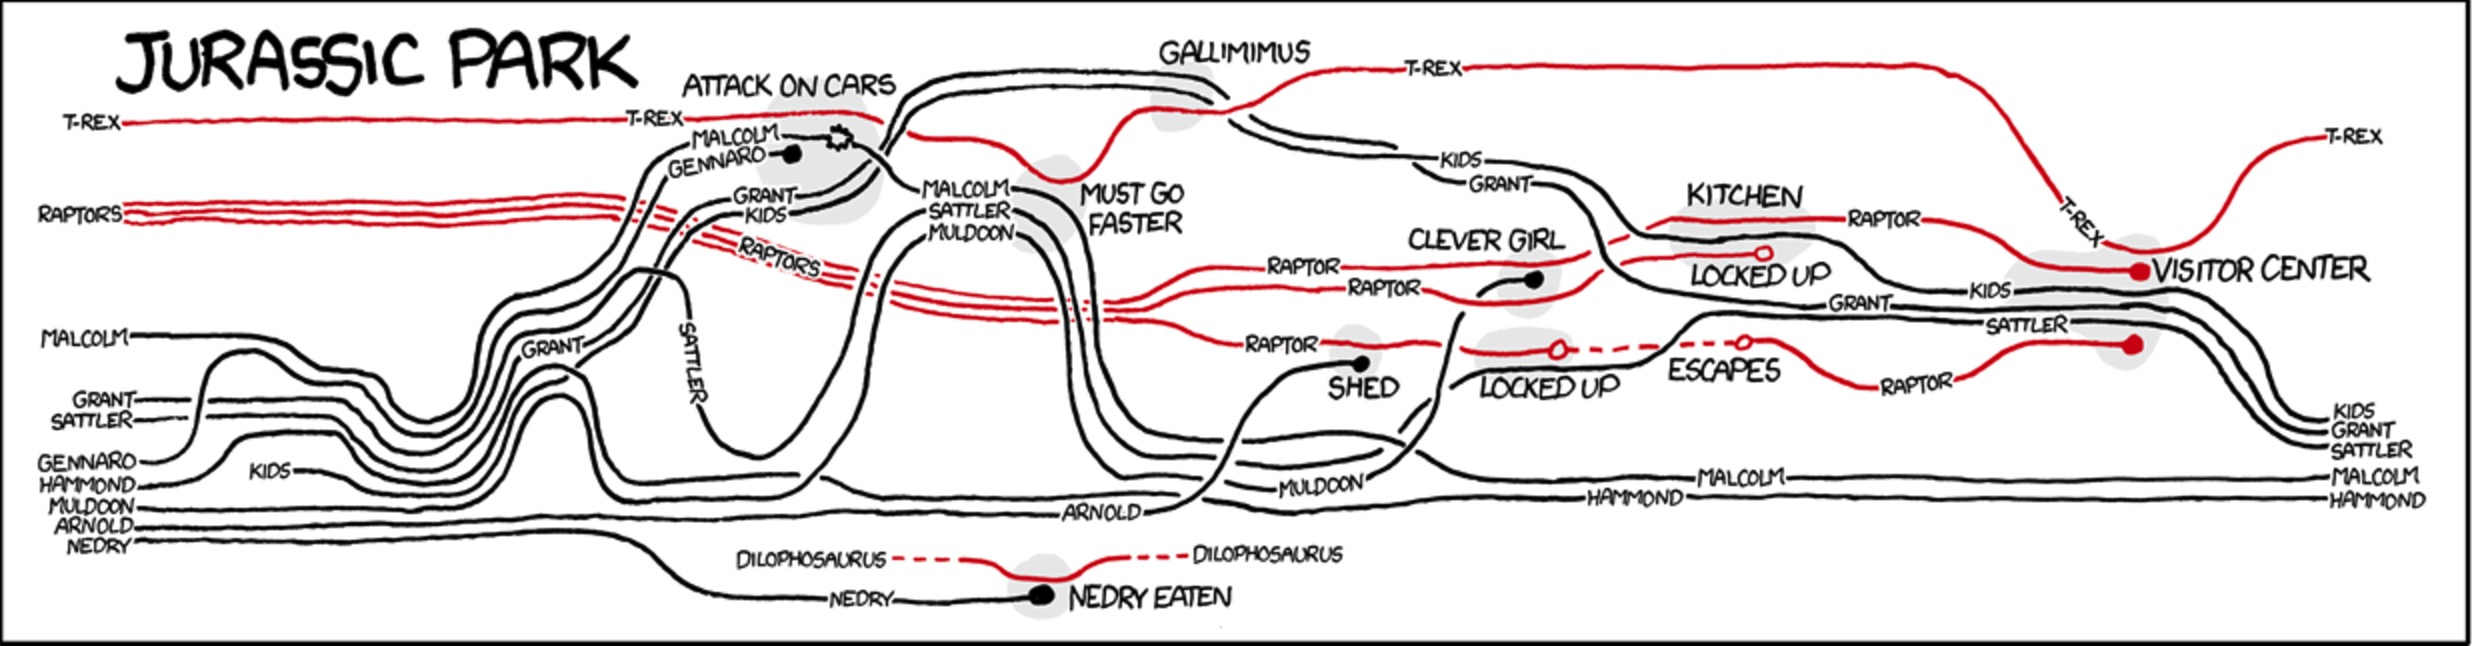
\includegraphics[width=15cm]{xkcd_jurassic_park}
	\caption{Jurassic park 人物关系叙事图,X轴表示时间,每个线条分别代表一个角色}
	\label{xkcd}
\end{figure}
% END == XKCD 手绘图


\subsection{相关研究}
@Todo 介绍 storyline 出现之前的一些展现故事的可视化方法,以及由 storyline 延伸来的可视化方法。

\subsection{设计原则}
在介绍 storyline 的设计准则之前,我们首先定义 storyline 中最基本的一对映射关系:
\begin{itemize}
\item \textbf{角色(Character 或 Entity)}
\item \textbf{线条(Thread)}
\end{itemize}
\textbf{Character} 是指故事中出现的人物或其他个体。新闻语料中,角色可以是人物、组织机构、国家等命名实体,它们一起构成了新闻故事六要素(时间、地点、人物、起因、经过和结果)之一的人物。电影、小说和新闻事件等通常都会有一个\textbf{主角(Leading Character)} 和若干的\textbf{配角(Ordinary Character)},所有的故事都围绕着主角展开和发展,并通过配角来充实整个故事。为了将故事中的 \textbf{Characters} 以及它们之间发生的事件映射到 storyline 中,便得到了 storyline 设计的基本原则:
\begin{itemize}
\item 水平轴上从左往右的\textbf{线条}表示故事中一个\textbf{角色}完整的生命周期。
\item 多个 \textbf{线条} 在某一时间段聚拢到一块,表示有这些\textbf{角色}共同参与了一个事件。线条之间的\textbf{收敛}和\textbf{发散}分别表示角色间的事件的开始和结束。
\end{itemize}
\textbf{Thread} 作为 \textbf{Characters} 的载体,每一个 \textbf{Thread}  都可以看作是故事的维度,一个由 \textbf{Threads} 组成的集合以及它们之间的位置随时间的变化(如:\textbf{收敛 Convergence},\textbf{发散 Divergence} 和\textbf{交叉 Intersection})描述了整个故事的发展变化。以上设计原则可以指导我们设计出更美观且易于理解的图形,因此被许多研究者广泛采用\cite{Ogawa:2010, Kim:2010},并在构建特定领域的 storyline 上获得了一定程度上的成功。然而,这些以上原则并没有很好的将文本的上下文信息(如,位置)表现出来。为了更好的描述事件发生的位置信息,Tanahashi 和 Ma \cite{tanahashi2012design} 在storyline 中用一个封闭的轮廓线作为背景将事件圈起来,并用不同的颜色表示不同的事件。同时为了让 storyline 展现得更加美观并增强可读性,Tanahashi 和 Ma 还添加了一条新的标准:
\begin{itemize}
\item 线条只有在收敛和发散的时候才可以偏离原始的方向。
\end{itemize}
也就是说,要尽可能让线条保持直线,减少线条的摆动。本文中,我们将采用以上这些原则来设计我们的 storyline。

\subsection{最优化度量}
\label{metrics}
给定一个角色(实体,人物)的集合以及它们之间在时间上的关联关系,我们的目标是要构建出一个美观且易于理解的 storyline 可视化图形。图形布局的构建可以分解为一系列的最优化求解问题,在我们的布局最优化方法中,我们采用 Tanahashi 和 Ma \cite{tanahashi2012design} 提出的最优化度量标准来定义我们的优化目标。
\begin{itemize}
\item \textbf{线条交叉 Line Crossovers}:最小化线条交叉的数量。
\item \textbf{线条摆动 Line Wiggles}:增强线条的笔直和连续性。
\item \textbf{空白距离 White Space Gaps}:最小化空白空间之间的距离,增强紧凑度。
\end{itemize}
很显然\textbf{线条交叉}容易造成图形的混乱,所以应该最小化交叉的数量。\textbf{线条摆动}是指线条偏离了原始的方向,这会打断线条的连续性,因此减少线条摆动次数可以增强可读性。\textbf{空白距离}是指图形中两个可视元素之间的空白空间的大小,空白空间是图形中区分元素的必要组成部分,然后过度的距离不仅容易造成空间的浪费,更重要的是容易让读者误以为这是上下文中角色之间的语意距离,所以也应当减少不必要的空白空间。

\section{Storyline 元素定义}
在 Storyline 的可视化中用到的数据最基本的形式就是各个角色之间按时间先后顺序排列的交互列表。这些角色之间的一系列交互可以被拆分成一系列\textbf{会话 Session},每个\textbf{会话}代表了一个时间跨度以及这段时间内有交互的角色集合。严格意义上,我们可以将\textbf{会话}定义为包含以下元素的基本单元:
\begin{itemize}
\item \textbf{起始时间}
\item \textbf{时间跨度}
\item \textbf{成员列表}
\end{itemize}
\textbf{起始时间}表示\textbf{会话}从何时开始,\textbf{时间跨度}表示该\textbf{会话}的持续时间,\textbf{成员列表}是指参与本次\textbf{会话}的所有角色的集合。
\subsection{Storyline 可视化元素定义}
在 storyline 中可视化元素包括: \textbf{线条},\textbf{角色标签},\textbf{节点}和\textbf{会话框}。针对每一个可视化元素,他们分别包含了多种呈现方式。
\begin{itemize}
\item \textbf{线条}。颜色,为了便于区分不同角色,每个线条的颜色必须与和它相邻的线条不同,最好的情况时保证所有线条的颜色均不相同;宽度,所有线条的宽度都一样。
\item \textbf{角色标签}。为了便于理解不同线条所代表的角色,角色标签将出现在线条的起点和终点。
\item \textbf{节点}。线条中空心圆点表示角色的出现,实心圆点表示角色的消失。
\item \textbf{会话框}。会话框呈现不规则的封闭图形,并且用不同颜色作为背景。会话框需要将参与会话的线条都囊括在内,同时必须排除未参加该会话的线条。
\end{itemize}


\subsection{Storyline 数据格式定义}
% BEGIN == JSON Schema & Example
\begin{listing}
\begin{minted}[frame=single, framesep=2mm, tabsize=4]{js}
{
    "sessions": [
        {
            "id": 0,
            "start": 0,
            "duration": 5,
            "characters": [
                0,
                2
            ]
        }
        {
            "id": 1,
            "start": 5,
            "duration": 10,
            "characters": [
                0,
                3,
                10
            ]
        }
   ]
}
\end{minted}
\caption{JSON example} 
\label{json-example}
\end{listing}
% END == JSON Schema & Example

\section{Storyline 布局算法}
本章节我们主要介绍 storyline 布局设计中的一些思想和使用的相关算法。首先我们将这个实际的问题进行抽象化描述,并用数学公式进行问题定义。
\subsection{问题定义}
布局设计中我们的主要目标就是最小化 \ref{metrics} 小节中提出的三个度量指标:\textbf{Line Crossover number},\textbf{wiggle number},\textbf{white space gaps}。 显然这是一个解空间极大的优化问题,要设计一个方法能够同时最优化以上三个指标是一项很困难的任务。对于此类解空间太大而不能轻易求得全局最优解的问题,我们也可以采用\textbf{遗传算法}\cite{tanahashi2012design} 等来求得一个接近最优的解决方案。然而,遗传算法的不足是获得的局部最优解经常会比较差,并且容易造成\textbf{早熟收敛}[@Todo reference]的问题。

为了弥补遗传算法的不足,并缩小搜索空间,我们将最优化的过程分解成几个独立的子问题。每个子问题分别最优化 \ref{metrics} 小节中的一个度量指标。子问题处理的原则是重要指标优先处理,因为它们对最终的可视化效果影响最为严重,更重要的是,在优化后续指标时不能影响前一指标的效果。已有研究[@Todo reference]指出减少线条交叉是最重要的步骤,减少线条的摆动以及空白距离次之。基于此,我们将问题分解成以下三个步骤:
\begin{itemize}
\item \textbf{步骤1:减少线条交叉的数目。}影响线条交叉数目最直接的因素就是线条的排列顺序以及会话的位置,因此为了减少线条不必要的交叉数目,我们要做的就是调整他们在空间上的排序以及位置。
\item \textbf{步骤2:减少线条摆动的数目。}线条的摆动收到会话的位置的影响,因此要减少线条的摆动就要尽可能得将会话摆放在适当的位置。同时,保证在同一个时间段内独立的,没有参与任何会话的的线条保持直线。
\item \textbf{步骤3:减少空白空间的距离。}为了使生成的图片更加的美观并且让信息更好的传递,我们还需要连续的优化空间中的空白距离。
\end{itemize}
 
 [@Todo 画图说明以上三个步骤]
 从数学角度考虑,storyline 的布局可以看成是一个有层次关系的 DAG(Directed Acyclic Graph)图,如Figure \ref{storyline-dag}。图中的每个节点代表了一个会话,根据会话发生的时间,可以将节点分为不同的层次,每个层次表示事件发展的一个阶段。
 
\subsection{线条排序}

\subsection{线条对齐}
线条对齐主要是为了减少线条的摆动,让更多的线段保持在同一水平直线上,这样有利于读者跟踪角色随时间的变化,避免因线条的交叉和扭动,使得混淆线条与角色的关联关系。为了将这一问题量化,我们用以下的数学公式来表达:
\begin{equation}
\label{align-global}
E_{align} = max \sum_{t=1}^{n_t-1} H\left(t\right)
\end{equation}
其中$H\left(t\right)$表示时间段$t$和$t+1$之间对齐的线段的数目。对于同一个角色在两个相邻时间段内的两条线段$S_t$和$S_{t+1}$,我们用线段的起点和终点坐标定义定义线段,则:
\begin{subequations}
\begin{align}
	S_t & = <(x_i, y_i), (x_{i+1},y_{i+1})> \label{eq:segment-1}\\
	S_{t+1} & = <(x_{i+1}, y_{i+1}), (x_{i+2},y_{i+2})> \label{eq:segment-2}
\end{align}
\end{subequations}
如果该线条在时间段$t$和$t+1$之内保持对齐,那么必定能得到$y_i = y_{i+2}$;反之如果$y_i \neq y_{i+2}$,那么该线条在时间段$t$和$t+1$之内一定不对齐。

[@Todo 画图说明这两个线段的几种画法]

很显然,线段不对齐是因为它参与的会话与它的起始位置不在同一垂直位置上,因此为了使线段保持对齐,只需要调整会话位置。一旦会话的位置确定了,参与该会话的线条的位置也就确定了。公式 \ref{align-global} 的优化目标是使得所有时间段间的水平线段总和最多,是一个全局优化问题。根据上面的分析,我们可以将其转化为:
\begin{equation}
\label{align-local}
E_{align} = \sum_{t=1}^{n_t-1} max H\left(t\right)
\end{equation}
从而将问题转变为一个局部优化问题,优化每一个局部从而使得整体最优。我们的目标变为使得每个相邻时间段内的水平线段数目最多。

\subsection{空间压缩} 
\begin{equation}
min \sum_{i=1}^{n_e} \sum_j^{n_t-1} \left(y_{i,j} - y_{i, j+1} \right)^2 + \beta \sum_{i=1}^{n_e} \sum_{j=1}^{n_t} y_{i,j}^2
\end{equation}
\label{eq:compact}
其中
\begin{subequations}
\begin{align}
	y_{i_1,j} < y_{i_2, j} & \qquad \text{If  } S_{i_1,j} \prec S_{i_2,j}; \label{eq:compact-1}\\
	y_{i,j} = y_{i,j+1} & \qquad \text{If  } S_{i,j} \leftrightarrow S_{i+1, j}; \label{eq:compact-2}\\
	y_{i,j} - y_{i+1,j} = d_{in} & \qquad \text{If  } SID(S_{i,j}) = SID(S_{i+1}, j); \label{eq:compact-3}\\
	\left|y_{i,j} - y_{i+1,j}\right| \geq d_{out} & \qquad \text{If  } SID(S_{i,j}) \neq SID(S_{i+1}, j). \label{eq:compact-4}
\end{align}
\end{subequations}
上面的式子中$S_{i,j}$指表示角色$i$在时间$j$内的线段, $y_{i,j}$表示$S_{i,j}$的$y$轴的坐标值;$SID(S_{i,j})$指会话$S_{i,j}$的ID。公式 \label{eq:compact} 中的第一项是线条摆动的惩罚函数,第二项是空白空间的惩罚函数。$\beta$ 是这两项之间的一个平衡因子,在我们的实验中,我们取 $\beta = 1$。以上的四个约束条件分别表示:
\begin{itemize}
\item (\ref{eq:compact-1}) 线条顺序约束。如果线段$S_{i_1,j}$的顺序小于$S_{i_2,j}$(我们用$S_{i_1,j} \prec S_{i_2,j}$表示),那么线段$S_{i_1,j}$被放置在$S_{i_2,j}$的上面。
\item (\ref{eq:compact-2})
\item (\ref{eq:compact-3})
\item (\ref{eq:compact-4})
\end{itemize}








